\hspace{1.5cm}
Neste processo é extraído  as informações das imagens, com a finalidade de reconhecer padrões e objetos mapeando as áreas da superfícies terrestre. Na área de estudo foi utilizado as cores, como associação de classe (Água $\rightarrow$ \textcolor{blue}{Azul}, Água com sedimentos $\rightarrow$ \textcolor{aquamarine}{Aquamarine}, Vegetação $\rightarrow$ \textcolor{green}{Verde} e Urbanização $\rightarrow$ \textcolor{red}{Vermelho}). Este passo desenvolveu-se com a criação da \textbf{\textit{Region of Interess}} (ROI), conforme figura \ref{roi01}.
\begin{itemize}
\item \textbf{Basic Tools}
\begin{itemize}
\item \textbf{Region of Interess}\\
\item \textbf{Amostras}\\
\begin{tabular}{|c|c|c|}
\hline
Tipo & Polignos & Points\\
\hline
\colorbox{blue}{Água} & 22 & 1155 \\
\hline
\colorbox{aquamarine}{Água com sedimentos} & 23&1350\\
\hline
\colorbox{green}{Vegetação} & 22&1138\\
\hline
\colorbox{red}{Urbanização} \footnote{No processo foi considerado urbanização tanto as construções, bem como os solos expostos.} & 30&586\\
\hline
\end{tabular}
\end{itemize}
\begin{figure}[!htpb]
        \centering
        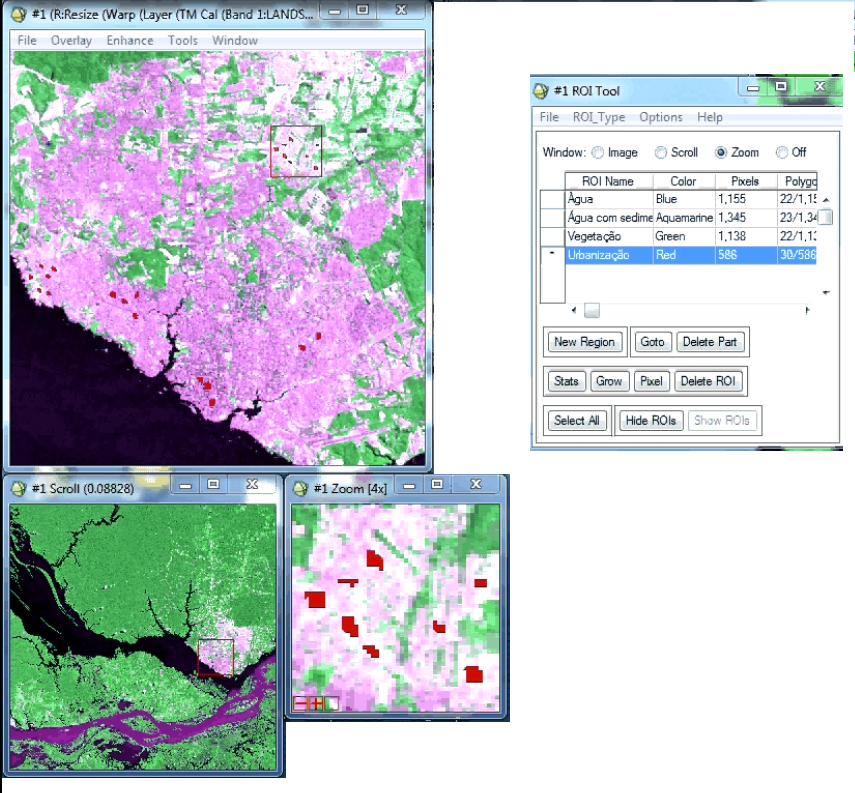
\includegraphics[scale =0.5]{imagens/roi01a.png}
        \caption{Geração das classes de Uso do Solo.}
        \label{roi01}
\end{figure}
\end{itemize}
\hspace{1.5cm}
Nosso processo de analise temporal será elaborado pelo modo supervisionado, mínima distancia. Este processo tem como primeira fase a coleta de amostra, das diversas classes. Aqui foi definido os tipos de classes do solo, para estudado, com suas respectivas cores.
\begin{itemize}
\item \textbf{Classification}
\begin{itemize}
\item \textbf{Supervised} $\rightarrow$ \textbf{Minimum Distance}\\
\end{itemize}
\begin{figure}[!htpb]
        \centering
        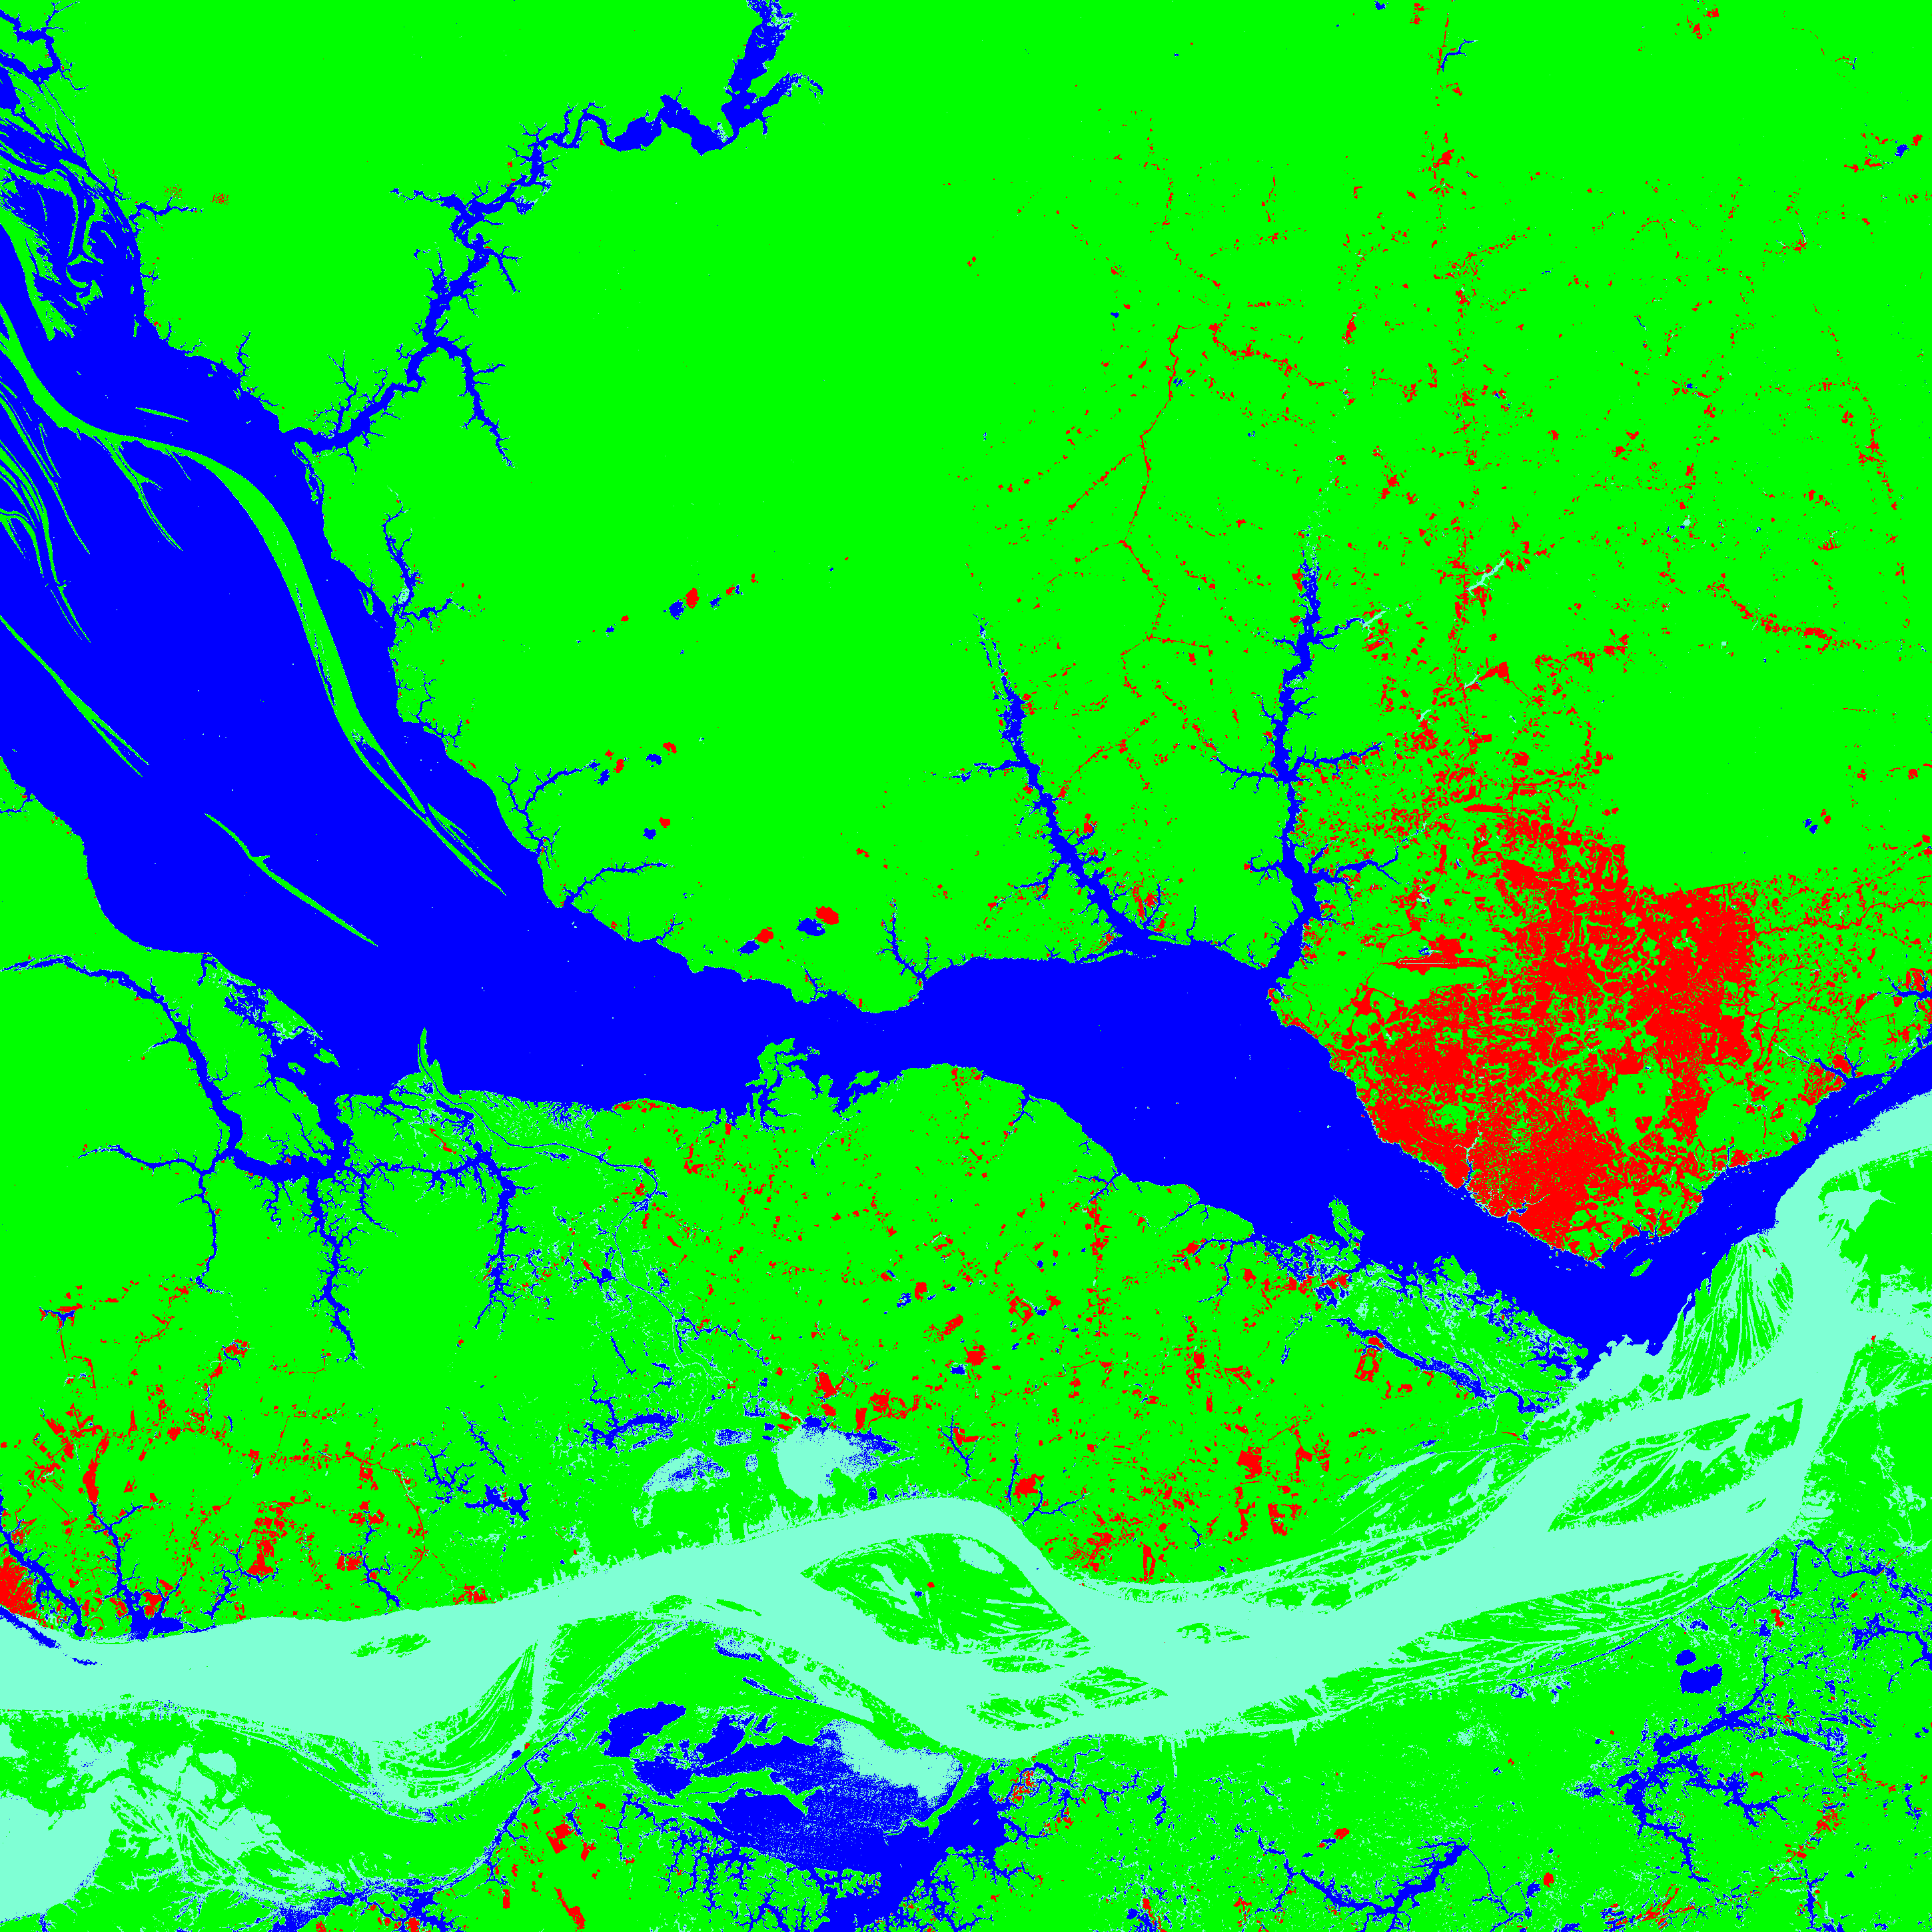
\includegraphics[scale =0.1]{imagens/1999_banda1a7_Class_MinDist.png}
        \caption{Geração das classes de Uso do Solo.}
        \label{1999}
        \centering
        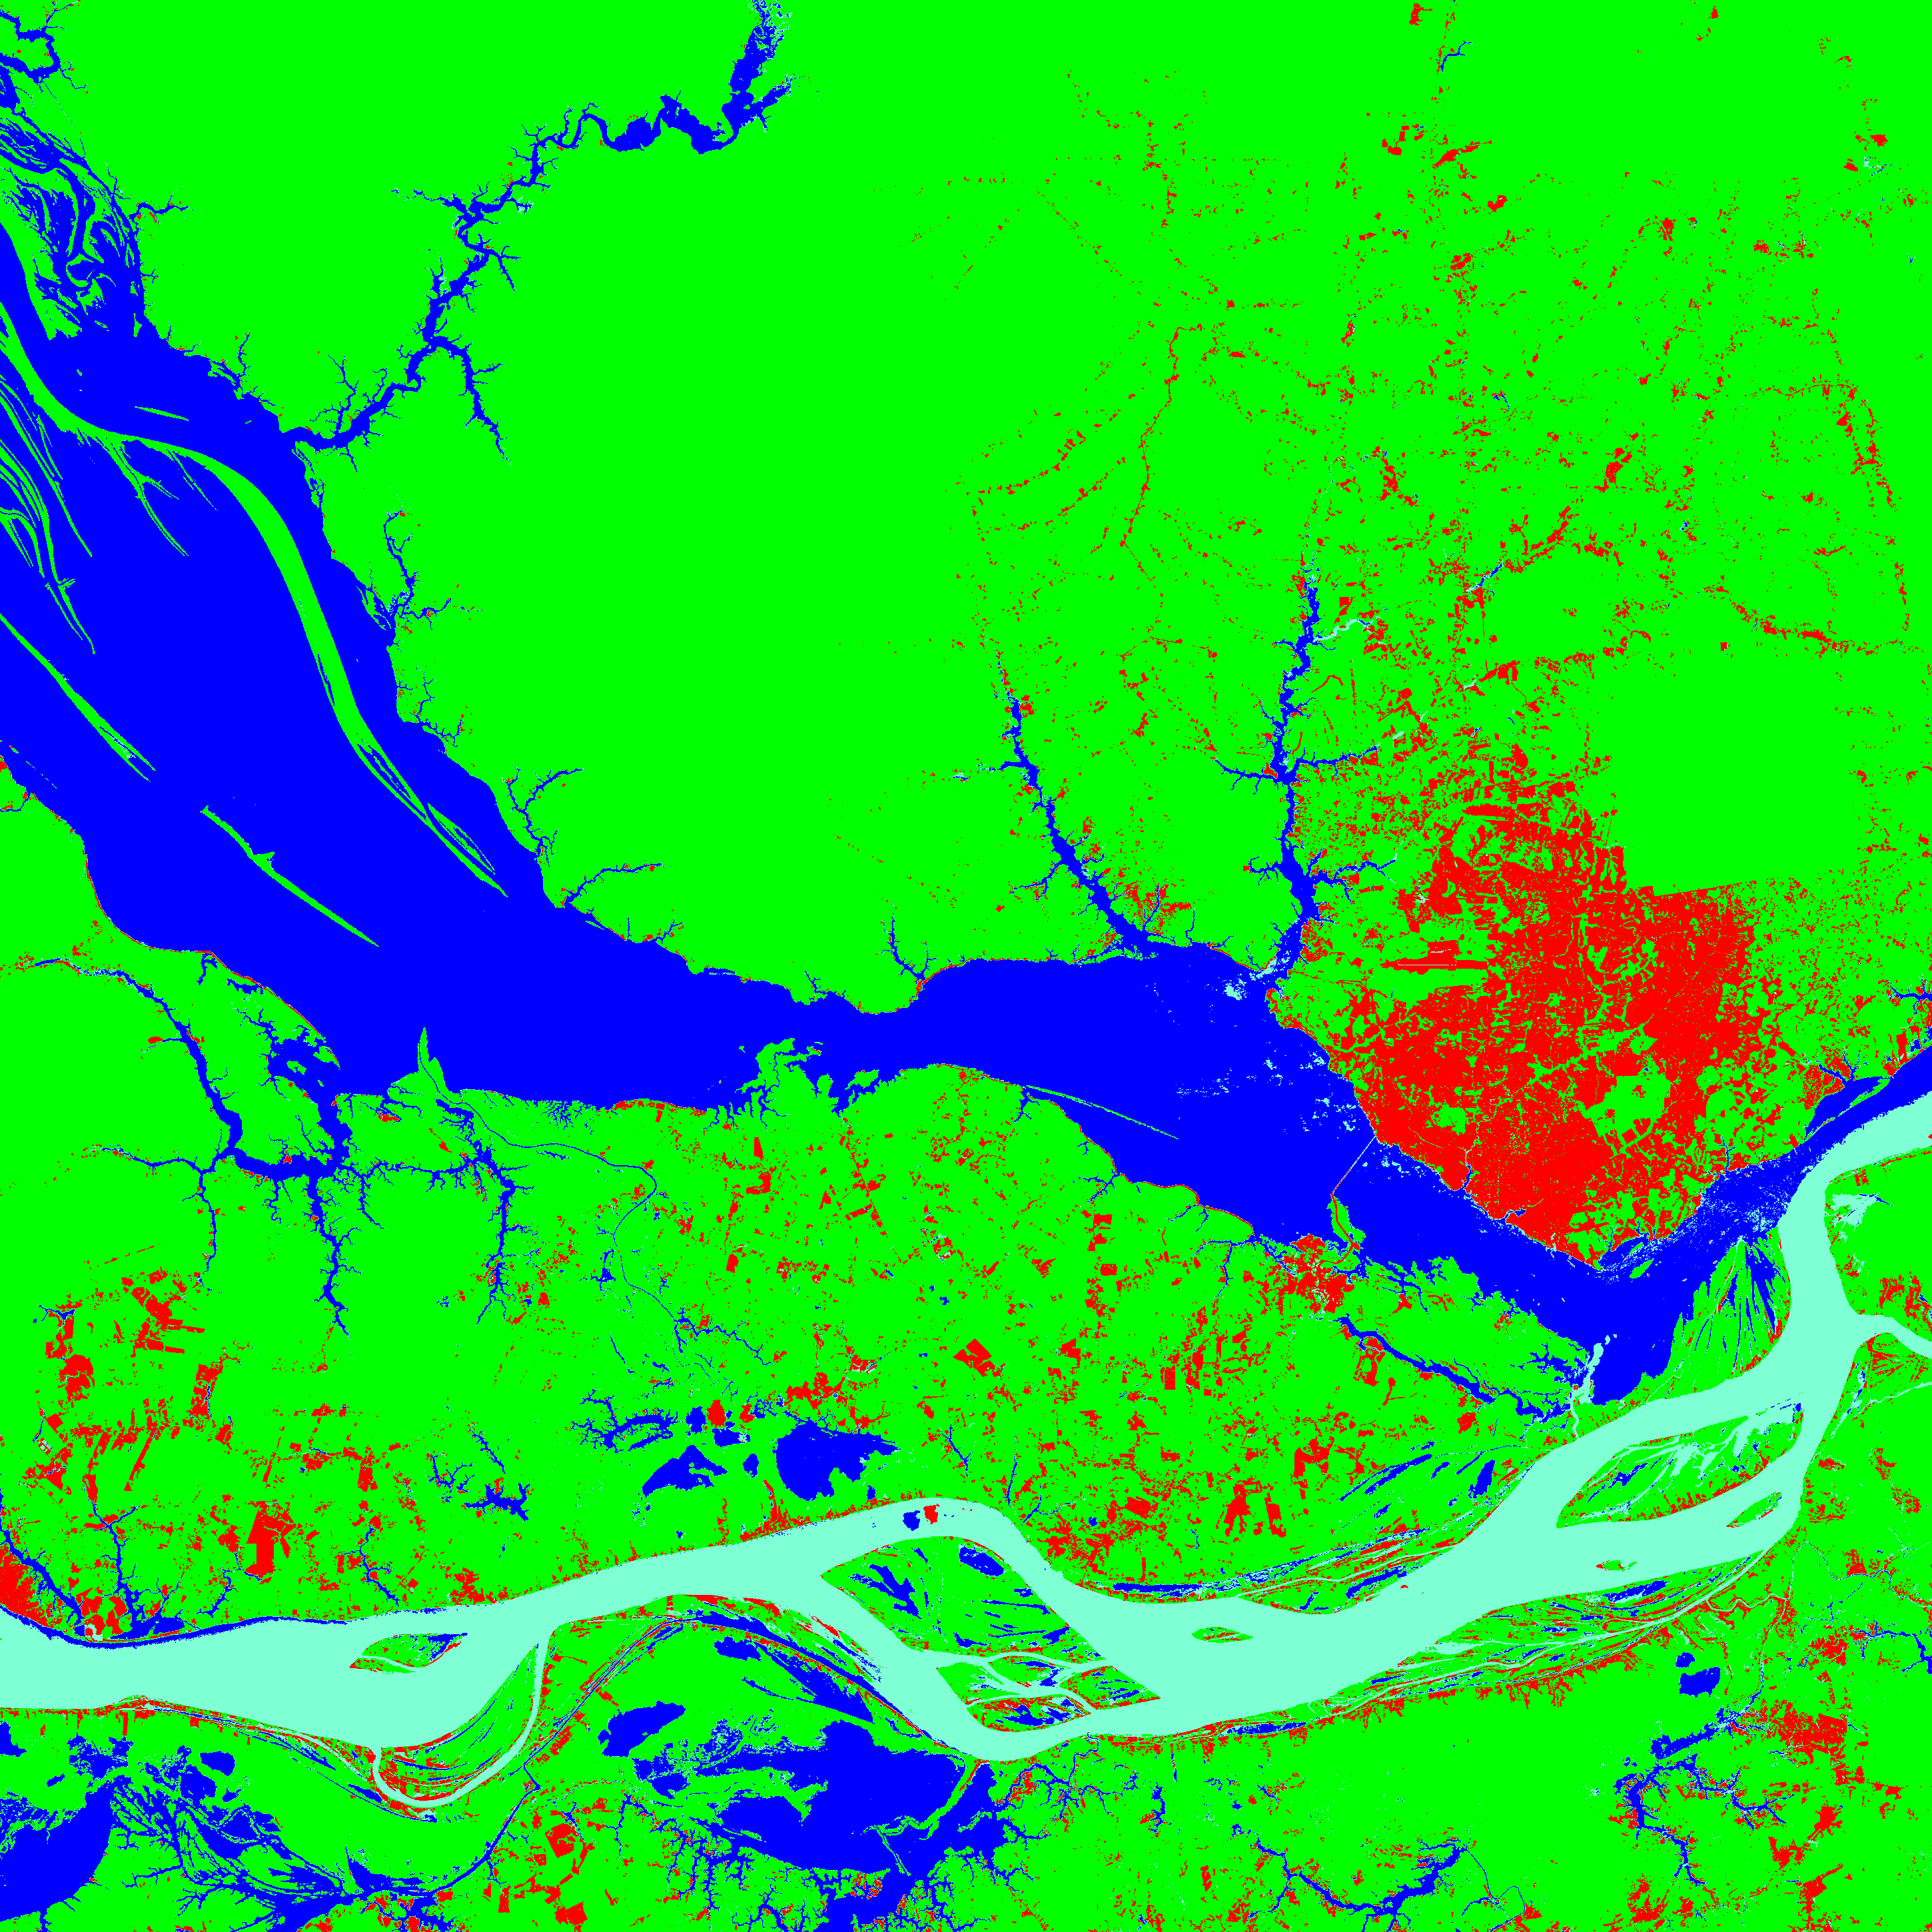
\includegraphics[scale =0.1]{imagens/2011_banda1a7_Class_MinDist.png}
        \caption{Geração das classes de Uso do Solo.}
        \label{2011}
\end{figure}
\end{itemize}
\hspace{1.5cm}
Esta técnica encontra os vetores desconhecido de cada classe, através dos calculos da distance Euclidean de cada vetor conhecido. Nas figuras ... e ... temos o resultado alcançado, para os anos de 1999 e 2011, respectivamente.

